\section{Task Specification}
In the first chapter it was pointed out that since it is nearly impossible to create intelligent system that would carry out all the creative processes, it is only reasonable to augment it by using the story designer's ``computational power''.
The task can be split in two parts:
\begin{enumerate}
\item Design the system, that will supplement some of the story designer's functionality. Later to be mentioned as \textbf{System0}.
\item Design the game development system (featuring other developers) in which \textit{System0} can function and be useful. This one will be called \textb{the development workflow}.
\end{enumerate}
\subsection{The development workflow}
To design \textit{System0's} it is firstly needed to understand the exact features this system needs to help other developers the most. For that let us analyze \textit{the development workflow} in detail.\par
As it was mentioned in the first section of chapter 1 , there are quite a few roles on the development team.
In \textit{the development workflow}, most of this people will exchange information with \textit{System0} in different points of time. Consider a couple of examples
\begin{example}
The only person who influences the result of a storyline creation is the story designer.  Other just process what was created. Each member has responsibilities shown below.
\begin{itemize}
 \item \textbf{storyline designer} provides the initial configuration to a storyline creating system (\textit{System0}). During the simulation one provides information requested by the system.
 \item \textbf{Level/World designer} designs the game world according to the output of \textit{System0}.
 \item \textbf{Game artist} provides essential content to the level designer.
 \item \textbf{Game designer} analyzes \textit{System0}'s output and then determines the optimal game mechanics. Afterwards, programmer creates the logical core of the future game and interprets the final story so it can be embedded into the game.
\end{itemize}
    \begin{figure}[h!]
     \begin{center}
      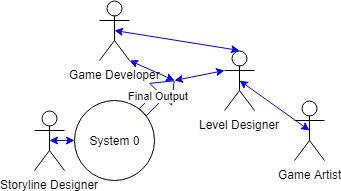
\includegraphics[width=400pt]{workflow_1}
      \caption{Example of game development interaction diagram \textnumero 1}
      \label{SimpleWorkflow}
     \end{center}
    \end{figure}
Dependencies between the developers are depicted on Fig. \ref{SimpleWorkflow}. Arrows represent data flow during the development process.
\end{example}

That is one of the least interactive examples. On the other side, there can be workflows, in which \textit{System0} is actively will communicate with every member of the development team.

\begin{example}
In this example,which is visualized in Figure \ref{RealWorkflow}, every team member exchanges data with \textit{System0}. The list of responsibilities changes as well.
\begin{itemize}
 \item \textbf{Storyline designer} does mostly the same actions.
 \item \textbf{Level/World designer} designs the world based on \textit{System0's} output, but this time one is given an ability to have an impact on \textit{System0's} result by specifying environmental details. For example, one can specify restrictions before the start of \textit{System0} or be questioned by \textit{System0} during the storyline creation.
 \item \textbf{Game artist} must provide the list of available content to \textit{System0}. Also can put several restrictions on the amount of the new content that can be added. For example, if artist already has a model of a bush and a tree, one can allow \textit{System0} to embed 2 random objects into the story that would need to be created by the artist afterwards.
 \item \textbf{Game Developer} can provide \textit{System0} with the information about the game mechanics to achieve more desirable output. That can be highly useful if the game's logical core is already written.
\end{description}
 \begin{figure}[h!]
    \begin{center}
      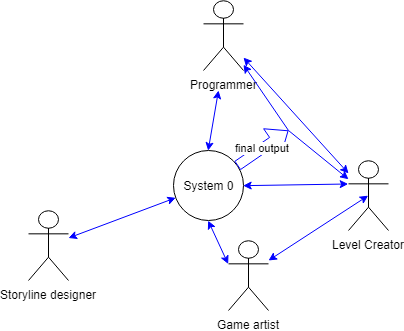
\includegraphics[width=400pt]{workflow_2}
      \caption{Example of game development interaction diagram \textnumero 2.}
      \label{RealWorkflow}
     \end{center}
    \end{figure}
This example closer resembles the real development process. The main reason to this is an ability to take into account the capabilities of each individual on the development team. In this case, \textit{System0}'s output can theoretically be an actual game. Also this example allows minimizing the dialogue between the story designer and \textit{System0}. The data retrieval process for \textit{System0} can be partially distributed among other members of the development team.
\end{example}\par
In conclusion, attempts of reducing the concept to a system with a concrete desired functions and parameters were not successful -- there are to many possible cases for such system to stay efficient. The diversity of possible uses makes it effective to design an expandable framework. This approach can result in an ability of end users to create a personalized system by filling it with required functionality.

